\documentclass[12pt,a4paper]{article}
\usepackage[utf8]{vietnam}
\usepackage{amsmath,amssymb}
\usepackage{tabularx}
\usepackage{tikz}
\usepackage{xcolor}
\usepackage[top=0.6cm, bottom=0.6cm, left=0.6cm, right=0.6cm]{geometry}
\usepackage[dethi]{ex_test}

\SAOPTN{widthSA=2.6,heightSA=0.62}

\setlength{\parskip}{0pt}

% Dòng kẻ chấm mờ đều đặn chuẩn viết tay (khoảng cách 6.5mm rộng rãi vừa vặn)
\newcommand{\dongke}[1]{%
  \begingroup%
  \setlength{\parskip}{0pt}%
  \baselineskip=18.5pt%
  \vspace{1.0mm}%
  \foreach \i in {1,...,#1}{%
    \noindent{\color{gray!60}\dotfill}\par%
  }%
  \vspace{0.6mm}%
  \endgroup%
}

% Khu vực bài làm chia 2 cột có vách ngăn mờ ở giữa
\newcommand{\dongkeHaiCot}[1]{%
  \par\vspace{0.5mm}%
  \noindent%
  \begin{minipage}[t]{0.485\linewidth}%
    \dongke{#1}%
  \end{minipage}%
  \hfill%
  {\color{gray!60}\vrule}%
  \hfill%
  \begin{minipage}[t]{0.485\linewidth}%
    \dongke{#1}%
  \end{minipage}%
}

% Định nghĩa ô bài tập tự luận trong bảng
\newcommand{\oBaiTap}[3][5]{%
  \vspace{1.0mm}%
  \noindent\textbf{#2} #3\par%
  \dongke{#1}%
}

\begin{document}
\pagestyle{empty}
% =============================================================================
% ========================= TOÁN 7 - TUẦN 08 - BUỔI 02: MÃ ĐỀ 101 =============
% ========================= MẶT TRƯỚC (TRANG 1/2) ==============================
% =============================================================================

\noindent
\begin{tabularx}{\linewidth}{|X|c|}
\hline
\textbf{PHIẾU KIỂM TRA ĐỊNH KỲ TOÁN 7 - TUẦN 08 - BUỔI 02} & \textbf{Mã đề: 101 - Trang 1/2} \\
\hline
\end{tabularx}

\vspace{1.2mm}

\noindent
\begin{tabularx}{\linewidth}{|p{3.2cm}|X|}
\hline
\centering\textbf{ĐIỂM SỐ} & \centering\textbf{LỜI NHẬN XÉT CỦA THẦY CÔ} \tabularnewline
\hline
\rule{0pt}{1.8cm} & \tabularnewline
\hline
\end{tabularx}

\vspace{1.5mm}

\noindent\textbf{Câu 1 (0,25 điểm).} Giá trị của biểu thức $\left(-\frac{2}{3}\right)^2$ bằng: \shortans{\frac{4}{9}}\par\vspace{2.4mm}
\noindent\textbf{Câu 2 (0,25 điểm).} Số đối của số thực $-\sqrt{7}$ là: \shortans{\sqrt{7}}\par\vspace{2.4mm}
\noindent\textbf{Câu 3 (0,25 điểm).} Giá trị của biểu thức $\sqrt{121}$ bằng: \shortans{11}\par\vspace{2.4mm}
\noindent\textbf{Câu 4 (0,25 điểm).} Giá trị của biểu thức $|-3{,}8| - |1{,}8|$ bằng: \shortans{2}\par\vspace{2.4mm}
\noindent\textbf{Câu 5 (0,25 điểm).} Làm tròn số thập phân $35{,}746$ đến hàng phần trăm: \shortans{35{,}75}\par\vspace{2.4mm}
\noindent\textbf{Câu 6 (0,25 điểm).} Hai góc kề bù có một góc bằng $65^\circ$. Góc còn lại có số đo là: \shortans{115^\circ}\par\vspace{2.4mm}
\noindent\textbf{Câu 7 (0,25 điểm).} Hai đường thẳng cắt nhau tạo góc $70^\circ$. Góc đối đỉnh với nó có số đo là: \shortans{70^\circ}\par\vspace{2.4mm}
\noindent\textbf{Câu 8 (0,25 điểm).} Cho hai đường thẳng $a \perp c$ và $b \perp c$. Quan hệ giữa $a$ và $b$ là: \shortans{\text{song song}}\par\vspace{2.4mm}
\noindent\textbf{Câu 9 (0,25 điểm).} Cho $a \parallel b$. Một góc so le trong với góc $50^\circ$ có số đo là: \shortans{50^\circ}\par\vspace{2.4mm}
\noindent\textbf{Câu 10 (0,25 điểm).} Một áo phông giá $120\,000$ đ, giảm giá $10\%$. Số tiền được giảm là: \shortans{12\,000\text{ đ}}\par\vspace{2.4mm}
\vspace{0.4mm}

\noindent\textbf{Câu 11 (3,0 điểm). Thực hiện phép tính (hợp lý nếu có thể):}
\vspace{0.8mm}

\noindent
\begin{tabularx}{\linewidth}{|X|X|}
\hline
\oBaiTap[5]{a) (0,5 điểm)}{$\dfrac{3}{7} + \left(-\dfrac{5}{2}\right) + \dfrac{4}{7} + \dfrac{3}{2}$} & 
\oBaiTap[5]{b) (0,5 điểm)}{$\dfrac{21}{25} \cdot \dfrac{11}{13} + \dfrac{21}{25} \cdot \dfrac{2}{13} - \dfrac{21}{25}$} \\
\hline
\oBaiTap[5]{c) (0,5 điểm)}{$\left(-\dfrac{1}{2}\right)^2 \cdot 24 - 1{,}5 \cdot 4$} & 
\oBaiTap[5]{d) (0,5 điểm)}{$\sqrt{\dfrac{16}{9}} - \left|-\dfrac{1}{3}\right| + \sqrt{36}$} \\
\hline
\oBaiTap[5]{e) (0,5 điểm)}{$\dfrac{5}{6} - \left[\dfrac{1}{6} + \left(\dfrac{1}{2}\right)^2\right]$} & 
\oBaiTap[5]{f) (0,5 điểm)}{$\dfrac{9^2 \cdot 2^{10}}{16^2 \cdot 3^3}$} \\
\hline
\end{tabularx}

\newpage
% =============================================================================
% ========================= TOÁN 7 - TUẦN 08 - BUỔI 02: MÃ ĐỀ 101 =============
% ========================= MẶT SAU (TRANG 2/2) ================================
% =============================================================================

\noindent
\begin{tabularx}{\linewidth}{|X|c|}
\hline
\textbf{TOÁN 7 - TUẦN 08 - BUỔI 02} & \textbf{Mã đề: 101 - Trang 2/2} \\
\hline
\end{tabularx}

\vspace{1.5mm}

\noindent\textbf{Câu 12 (2,0 điểm). Tìm số hữu tỉ $x$, biết:}
\vspace{0.8mm}

\noindent
\begin{tabularx}{\linewidth}{|X|X|}
\hline
\oBaiTap[5]{a) (0,5 điểm)}{$x - \dfrac{1}{4} = \dfrac{3}{4}$} & 
\oBaiTap[5]{b) (0,5 điểm)}{$\dfrac{2}{3}x + \dfrac{1}{6} = \dfrac{3}{2}$} \\
\hline
\oBaiTap[5]{c) (0,5 điểm)}{$\left(x + \dfrac{1}{2}\right)^2 = \dfrac{25}{4}$} & 
\oBaiTap[5]{d) (0,5 điểm)}{$|2x - 1| = 5$} \\
\hline
\end{tabularx}

\vspace{1.5mm}

\noindent
\begin{tabularx}{\linewidth}{|X|}
\hline
\vspace{0.5mm}
\begin{minipage}[t]{0.68\linewidth}
\vspace{0pt}
\textbf{Câu 13 (2,0 điểm).} Cho hình vẽ bên, biết đường thẳng $a \perp AB$ tại $A$ và $b \perp AB$ tại $B$. Đường thẳng $c$ cắt $a$ tại $C$ và cắt $b$ tại $D$ sao cho $\widehat{ACD} = 120^\circ$.\par\vspace{0.4mm}
\textbf{a) (1,0 điểm)} Chứng minh rằng đường thẳng $a$ song song với đường thẳng $b$ ($a \parallel b$).\par\vspace{0.4mm}
\textbf{b) (1,0 điểm)} Tính số đo góc $\widehat{CDB}$ và số đo góc kề bù với góc $\widehat{CDB}$.
\end{minipage}\hfill
\begin{minipage}[t]{0.30\linewidth}
\vspace{0pt}\centering
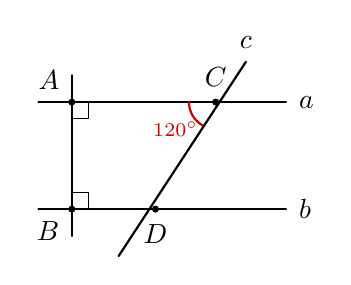
\begin{tikzpicture}[scale=0.85, >=stealth, line join=round, line cap=round]
  % Doan thang AB vuong goc
  \draw[thick] (0.8, 0.2) -- (0.8, 2.6);
  % Duong thang a qua A
  \draw[thick] (0.3, 2.2) -- (4.0, 2.2) node[right=1pt] {$a$};
  % Duong thang b qua B
  \draw[thick] (0.3, 0.6) -- (4.0, 0.6) node[right=1pt] {$b$};
  % Cat tuyen c
  \draw[thick] (3.4, 2.8) node[above=1pt] {$c$} -- (1.5, -0.1);
  
  % Giao diem A va B
  \fill (0.8, 2.2) circle (1.5pt) node[above left=1pt] {$A$};
  \fill (0.8, 0.6) circle (1.5pt) node[below left=1pt] {$B$};
  % Ky hieu vuong goc
  \draw (0.8, 1.95) -- (1.05, 1.95) -- (1.05, 2.2);
  \draw (0.8, 0.85) -- (1.05, 0.85) -- (1.05, 0.6);
  
  % Giao diem C va D
  \fill (2.95, 2.2) circle (1.5pt) node[above=2pt] {$C$};
  \fill (2.05, 0.6) circle (1.5pt) node[below=2pt] {$D$};
  
  % Goc tu ACD
  \draw[red!80!black, thick] (2.95, 2.2) ++(180:0.4) arc (180:240:0.4);
  \node[red!80!black, font=\scriptsize] at (2.35, 1.8) {$120^\circ$};
\end{tikzpicture}
\end{minipage}\par
\vspace{0.4mm}
\noindent\textit{Bài giải:}\dongkeHaiCot{10}
\\ \hline
\end{tabularx}

\vspace{1.5mm}

\noindent
\begin{tabularx}{\linewidth}{|X|}
\hline
\vspace{0.5mm}
\textbf{Câu 14 (0,5 điểm).} Cho biểu thức: $S = \dfrac{1}{3} + \dfrac{1}{3^2} + \dfrac{1}{3^3} + \dots + \dfrac{1}{3^{2026}}$. Chứng minh rằng $S < \dfrac{1}{2}$.\par
\vspace{0.4mm}
\noindent\textit{Bài giải:}\dongkeHaiCot{6}
\\ \hline
\end{tabularx}

\newpage
% =============================================================================
% ========================= TOÁN 7 - TUẦN 08 - BUỔI 02: MÃ ĐỀ 102 =============
% ========================= MẶT TRƯỚC (TRANG 1/2) ==============================
% =============================================================================

\noindent
\begin{tabularx}{\linewidth}{|X|c|}
\hline
\textbf{PHIẾU KIỂM TRA ĐỊNH KỲ TOÁN 7 - TUẦN 08 - BUỔI 02} & \textbf{Mã đề: 102 - Trang 1/2} \\
\hline
\end{tabularx}

\vspace{1.2mm}

\noindent
\begin{tabularx}{\linewidth}{|p{3.2cm}|X|}
\hline
\centering\textbf{ĐIỂM SỐ} & \centering\textbf{LỜI NHẬN XÉT CỦA THẦY CÔ} \tabularnewline
\hline
\rule{0pt}{1.8cm} & \tabularnewline
\hline
\end{tabularx}

\vspace{1.5mm}

\noindent\textbf{Câu 1 (0,25 điểm).} Giá trị của biểu thức $\left(-\frac{3}{2}\right)^2$ bằng: \shortans{\frac{9}{4}}\par\vspace{2.4mm}
\noindent\textbf{Câu 2 (0,25 điểm).} Số đối của số thực $-\sqrt{5}$ là: \shortans{\sqrt{5}}\par\vspace{2.4mm}
\noindent\textbf{Câu 3 (0,25 điểm).} Giá trị của biểu thức $\sqrt{144}$ bằng: \shortans{12}\par\vspace{2.4mm}
\noindent\textbf{Câu 4 (0,25 điểm).} Giá trị của biểu thức $|-4{,}6| - |1{,}6|$ bằng: \shortans{3}\par\vspace{2.4mm}
\noindent\textbf{Câu 5 (0,25 điểm).} Làm tròn số thập phân $48{,}263$ đến hàng phần trăm: \shortans{48{,}26}\par\vspace{2.4mm}
\noindent\textbf{Câu 6 (0,25 điểm).} Hai góc kề bù có một góc bằng $75^\circ$. Góc còn lại có số đo là: \shortans{105^\circ}\par\vspace{2.4mm}
\noindent\textbf{Câu 7 (0,25 điểm).} Hai đường thẳng cắt nhau tạo góc $80^\circ$. Góc đối đỉnh với nó có số đo là: \shortans{80^\circ}\par\vspace{2.4mm}
\noindent\textbf{Câu 8 (0,25 điểm).} Cho $a \parallel b$ và đường thẳng $c \perp a$. Quan hệ giữa $c$ và $b$ là: \shortans{\text{vuông góc}}\par\vspace{2.4mm}
\noindent\textbf{Câu 9 (0,25 điểm).} Cho $a \parallel b$. Một góc đồng vị với góc $55^\circ$ có số đo là: \shortans{55^\circ}\par\vspace{2.4mm}
\noindent\textbf{Câu 10 (0,25 điểm).} Một cuốn sách giá $60\,000$ đ, giảm giá $20\%$. Số tiền được giảm là: \shortans{12\,000\text{ đ}}\par\vspace{2.4mm}
\vspace{0.4mm}

\noindent\textbf{Câu 11 (3,0 điểm). Thực hiện phép tính (hợp lý nếu có thể):}
\vspace{0.8mm}

\noindent
\begin{tabularx}{\linewidth}{|X|X|}
\hline
\oBaiTap[5]{a) (0,5 điểm)}{$\dfrac{2}{9} + \left(-\dfrac{7}{3}\right) + \dfrac{7}{9} + \dfrac{4}{3}$} & 
\oBaiTap[5]{b) (0,5 điểm)}{$\dfrac{19}{24} \cdot \dfrac{8}{11} + \dfrac{19}{24} \cdot \dfrac{3}{11} - \dfrac{19}{24}$} \\
\hline
\oBaiTap[5]{c) (0,5 điểm)}{$\left(-\dfrac{1}{3}\right)^2 \cdot 27 - 0{,}75 \cdot 4$} & 
\oBaiTap[5]{d) (0,5 điểm)}{$\sqrt{\dfrac{25}{4}} - \left|-\dfrac{3}{2}\right| + \sqrt{49}$} \\
\hline
\oBaiTap[5]{e) (0,5 điểm)}{$\dfrac{7}{8} - \left[\dfrac{1}{8} + \left(\dfrac{1}{2}\right)^3\right]$} & 
\oBaiTap[5]{f) (0,5 điểm)}{$\dfrac{4^3 \cdot 27^2}{8^2 \cdot 9^2}$} \\
\hline
\end{tabularx}

\newpage
% =============================================================================
% ========================= TOÁN 7 - TUẦN 08 - BUỔI 02: MÃ ĐỀ 102 =============
% ========================= MẶT SAU (TRANG 2/2) ================================
% =============================================================================

\noindent
\begin{tabularx}{\linewidth}{|X|c|}
\hline
\textbf{TOÁN 7 - TUẦN 08 - BUỔI 02} & \textbf{Mã đề: 102 - Trang 2/2} \\
\hline
\end{tabularx}

\vspace{1.5mm}

\noindent\textbf{Câu 12 (2,0 điểm). Tìm số hữu tỉ $x$, biết:}
\vspace{0.8mm}

\noindent
\begin{tabularx}{\linewidth}{|X|X|}
\hline
\oBaiTap[5]{a) (0,5 điểm)}{$x - \dfrac{1}{3} = \dfrac{2}{3}$} & 
\oBaiTap[5]{b) (0,5 điểm)}{$\dfrac{3}{5}x + \dfrac{1}{10} = \dfrac{13}{10}$} \\
\hline
\oBaiTap[5]{c) (0,5 điểm)}{$\left(x + \dfrac{1}{3}\right)^2 = \dfrac{49}{9}$} & 
\oBaiTap[5]{d) (0,5 điểm)}{$|3x - 1| = 8$} \\
\hline
\end{tabularx}

\vspace{1.5mm}

\noindent
\begin{tabularx}{\linewidth}{|X|}
\hline
\vspace{0.5mm}
\begin{minipage}[t]{0.68\linewidth}
\vspace{0pt}
\textbf{Câu 13 (2,0 điểm).} Cho hình vẽ bên, biết đường thẳng $a \perp AB$ tại $A$ và $b \perp AB$ tại $B$. Đường thẳng $c$ cắt $a$ tại $C$ và cắt $b$ tại $D$ sao cho $\widehat{ACD} = 130^\circ$.\par\vspace{0.4mm}
\textbf{a) (1,0 điểm)} Chứng minh rằng đường thẳng $a$ song song với đường thẳng $b$ ($a \parallel b$).\par\vspace{0.4mm}
\textbf{b) (1,0 điểm)} Tính số đo góc $\widehat{CDB}$ và số đo góc kề bù với góc $\widehat{CDB}$.
\end{minipage}\hfill
\begin{minipage}[t]{0.30\linewidth}
\vspace{0pt}\centering
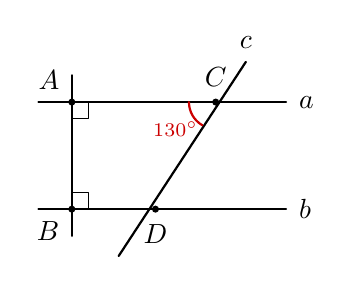
\begin{tikzpicture}[scale=0.85, >=stealth, line join=round, line cap=round]
  % Doan thang AB vuong goc
  \draw[thick] (0.8, 0.2) -- (0.8, 2.6);
  % Duong thang a qua A
  \draw[thick] (0.3, 2.2) -- (4.0, 2.2) node[right=1pt] {$a$};
  % Duong thang b qua B
  \draw[thick] (0.3, 0.6) -- (4.0, 0.6) node[right=1pt] {$b$};
  % Cat tuyen c
  \draw[thick] (3.4, 2.8) node[above=1pt] {$c$} -- (1.5, -0.1);
  
  % Giao diem A va B
  \fill (0.8, 2.2) circle (1.5pt) node[above left=1pt] {$A$};
  \fill (0.8, 0.6) circle (1.5pt) node[below left=1pt] {$B$};
  % Ky hieu vuong goc
  \draw (0.8, 1.95) -- (1.05, 1.95) -- (1.05, 2.2);
  \draw (0.8, 0.85) -- (1.05, 0.85) -- (1.05, 0.6);
  
  % Giao diem C va D
  \fill (2.95, 2.2) circle (1.5pt) node[above=2pt] {$C$};
  \fill (2.05, 0.6) circle (1.5pt) node[below=2pt] {$D$};
  
  % Goc tu ACD
  \draw[red!80!black, thick] (2.95, 2.2) ++(180:0.4) arc (180:240:0.4);
  \node[red!80!black, font=\scriptsize] at (2.35, 1.8) {$130^\circ$};
\end{tikzpicture}
\end{minipage}\par
\vspace{0.4mm}
\noindent\textit{Bài giải:}\dongkeHaiCot{10}
\\ \hline
\end{tabularx}

\vspace{1.5mm}

\noindent
\begin{tabularx}{\linewidth}{|X|}
\hline
\vspace{0.5mm}
\textbf{Câu 14 (0,5 điểm).} Cho biểu thức: $S = \dfrac{1}{4} + \dfrac{1}{4^2} + \dfrac{1}{4^3} + \dots + \dfrac{1}{4^{2026}}$. Chứng minh rằng $S < \dfrac{1}{3}$.\par
\vspace{0.4mm}
\noindent\textit{Bài giải:}\dongkeHaiCot{6}
\\ \hline
\end{tabularx}

\newpage
% =============================================================================
% ========================= TOÁN 7 - TUẦN 08 - BUỔI 02: MÃ ĐỀ 103 =============
% ========================= MẶT TRƯỚC (TRANG 1/2) ==============================
% =============================================================================

\noindent
\begin{tabularx}{\linewidth}{|X|c|}
\hline
\textbf{PHIẾU KIỂM TRA ĐỊNH KỲ TOÁN 7 - TUẦN 08 - BUỔI 02} & \textbf{Mã đề: 103 - Trang 1/2} \\
\hline
\end{tabularx}

\vspace{1.2mm}

\noindent
\begin{tabularx}{\linewidth}{|p{3.2cm}|X|}
\hline
\centering\textbf{ĐIỂM SỐ} & \centering\textbf{LỜI NHẬN XÉT CỦA THẦY CÔ} \tabularnewline
\hline
\rule{0pt}{1.8cm} & \tabularnewline
\hline
\end{tabularx}

\vspace{1.5mm}

\noindent\textbf{Câu 1 (0,25 điểm).} Giá trị của biểu thức $\left(-\frac{1}{4}\right)^2$ bằng: \shortans{\frac{1}{16}}\par\vspace{2.4mm}
\noindent\textbf{Câu 2 (0,25 điểm).} Số đối của số thực $-\sqrt{11}$ là: \shortans{\sqrt{11}}\par\vspace{2.4mm}
\noindent\textbf{Câu 3 (0,25 điểm).} Giá trị của biểu thức $\sqrt{169}$ bằng: \shortans{13}\par\vspace{2.4mm}
\noindent\textbf{Câu 4 (0,25 điểm).} Giá trị của biểu thức $|-5{,}9| - |1{,}9|$ bằng: \shortans{4}\par\vspace{2.4mm}
\noindent\textbf{Câu 5 (0,25 điểm).} Làm tròn số thập phân $62{,}538$ đến hàng phần trăm: \shortans{62{,}54}\par\vspace{2.4mm}
\noindent\textbf{Câu 6 (0,25 điểm).} Hai góc kề bù có một góc bằng $55^\circ$. Góc còn lại có số đo là: \shortans{125^\circ}\par\vspace{2.4mm}
\noindent\textbf{Câu 7 (0,25 điểm).} Hai đường thẳng cắt nhau tạo góc $60^\circ$. Góc đối đỉnh với nó có số đo là: \shortans{60^\circ}\par\vspace{2.4mm}
\noindent\textbf{Câu 8 (0,25 điểm).} Hai đường thẳng phân biệt cùng song song với đường thứ ba thì: \shortans{\text{song song}}\par\vspace{2.4mm}
\noindent\textbf{Câu 9 (0,25 điểm).} Cho $a \parallel b$. Một góc trong cùng phía với góc $65^\circ$ có số đo là: \shortans{115^\circ}\par\vspace{2.4mm}
\noindent\textbf{Câu 10 (0,25 điểm).} Một chiếc ba lô giá $200\,000$ đ, giảm giá $15\%$. Số tiền được giảm là: \shortans{30\,000\text{ đ}}\par\vspace{2.4mm}
\vspace{0.4mm}

\noindent\textbf{Câu 11 (3,0 điểm). Thực hiện phép tính (hợp lý nếu có thể):}
\vspace{0.8mm}

\noindent
\begin{tabularx}{\linewidth}{|X|X|}
\hline
\oBaiTap[5]{a) (0,5 điểm)}{$\dfrac{4}{11} + \left(-\dfrac{9}{4}\right) + \dfrac{7}{11} + \dfrac{5}{4}$} & 
\oBaiTap[5]{b) (0,5 điểm)}{$\dfrac{16}{29} \cdot \dfrac{7}{15} + \dfrac{16}{29} \cdot \dfrac{8}{15} - \dfrac{16}{29}$} \\
\hline
\oBaiTap[5]{c) (0,5 điểm)}{$\left(-\dfrac{1}{2}\right)^3 \cdot (-32) - 2{,}5 \cdot 4$} & 
\oBaiTap[5]{d) (0,5 điểm)}{$\sqrt{\dfrac{49}{25}} - \left|-\dfrac{2}{5}\right| + \sqrt{81}$} \\
\hline
\oBaiTap[5]{e) (0,5 điểm)}{$\dfrac{11}{12} - \left[\dfrac{1}{4} + \left(\dfrac{1}{3}\right)^2 \cdot 3\right]$} & 
\oBaiTap[5]{f) (0,5 điểm)}{$\dfrac{8^3 \cdot 25^2}{4^4 \cdot 125}$} \\
\hline
\end{tabularx}

\newpage
% =============================================================================
% ========================= TOÁN 7 - TUẦN 08 - BUỔI 02: MÃ ĐỀ 103 =============
% ========================= MẶT SAU (TRANG 2/2) ================================
% =============================================================================

\noindent
\begin{tabularx}{\linewidth}{|X|c|}
\hline
\textbf{TOÁN 7 - TUẦN 08 - BUỔI 02} & \textbf{Mã đề: 103 - Trang 2/2} \\
\hline
\end{tabularx}

\vspace{1.5mm}

\noindent\textbf{Câu 12 (2,0 điểm). Tìm số hữu tỉ $x$, biết:}
\vspace{0.8mm}

\noindent
\begin{tabularx}{\linewidth}{|X|X|}
\hline
\oBaiTap[5]{a) (0,5 điểm)}{$x - \dfrac{2}{5} = \dfrac{3}{5}$} & 
\oBaiTap[5]{b) (0,5 điểm)}{$\dfrac{4}{7}x + \dfrac{3}{14} = \dfrac{19}{14}$} \\
\hline
\oBaiTap[5]{c) (0,5 điểm)}{$\left(x + \dfrac{1}{4}\right)^2 = \dfrac{81}{16}$} & 
\oBaiTap[5]{d) (0,5 điểm)}{$|2x - 3| = 5$} \\
\hline
\end{tabularx}

\vspace{1.5mm}

\noindent
\begin{tabularx}{\linewidth}{|X|}
\hline
\vspace{0.5mm}
\begin{minipage}[t]{0.68\linewidth}
\vspace{0pt}
\textbf{Câu 13 (2,0 điểm).} Cho hình vẽ bên, biết đường thẳng $a \perp AB$ tại $A$ và $b \perp AB$ tại $B$. Đường thẳng $c$ cắt $a$ tại $C$ và cắt $b$ tại $D$ sao cho $\widehat{ACD} = 115^\circ$.\par\vspace{0.4mm}
\textbf{a) (1,0 điểm)} Chứng minh rằng đường thẳng $a$ song song với đường thẳng $b$ ($a \parallel b$).\par\vspace{0.4mm}
\textbf{b) (1,0 điểm)} Tính số đo góc $\widehat{CDB}$ và số đo góc kề bù với góc $\widehat{CDB}$.
\end{minipage}\hfill
\begin{minipage}[t]{0.30\linewidth}
\vspace{0pt}\centering
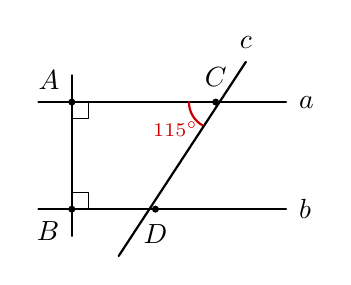
\begin{tikzpicture}[scale=0.85, >=stealth, line join=round, line cap=round]
  % Doan thang AB vuong goc
  \draw[thick] (0.8, 0.2) -- (0.8, 2.6);
  % Duong thang a qua A
  \draw[thick] (0.3, 2.2) -- (4.0, 2.2) node[right=1pt] {$a$};
  % Duong thang b qua B
  \draw[thick] (0.3, 0.6) -- (4.0, 0.6) node[right=1pt] {$b$};
  % Cat tuyen c
  \draw[thick] (3.4, 2.8) node[above=1pt] {$c$} -- (1.5, -0.1);
  
  % Giao diem A va B
  \fill (0.8, 2.2) circle (1.5pt) node[above left=1pt] {$A$};
  \fill (0.8, 0.6) circle (1.5pt) node[below left=1pt] {$B$};
  % Ky hieu vuong goc
  \draw (0.8, 1.95) -- (1.05, 1.95) -- (1.05, 2.2);
  \draw (0.8, 0.85) -- (1.05, 0.85) -- (1.05, 0.6);
  
  % Giao diem C va D
  \fill (2.95, 2.2) circle (1.5pt) node[above=2pt] {$C$};
  \fill (2.05, 0.6) circle (1.5pt) node[below=2pt] {$D$};
  
  % Goc tu ACD
  \draw[red!80!black, thick] (2.95, 2.2) ++(180:0.4) arc (180:240:0.4);
  \node[red!80!black, font=\scriptsize] at (2.35, 1.8) {$115^\circ$};
\end{tikzpicture}
\end{minipage}\par
\vspace{0.4mm}
\noindent\textit{Bài giải:}\dongkeHaiCot{10}
\\ \hline
\end{tabularx}

\vspace{1.5mm}

\noindent
\begin{tabularx}{\linewidth}{|X|}
\hline
\vspace{0.5mm}
\textbf{Câu 14 (0,5 điểm).} Cho biểu thức: $S = \dfrac{1}{5} + \dfrac{1}{5^2} + \dfrac{1}{5^3} + \dots + \dfrac{1}{5^{2026}}$. Chứng minh rằng $S < \dfrac{1}{4}$.\par
\vspace{0.4mm}
\noindent\textit{Bài giải:}\dongkeHaiCot{6}
\\ \hline
\end{tabularx}

\newpage
% =============================================================================
% ========================= TOÁN 7 - TUẦN 08 - BUỔI 02: MÃ ĐỀ 104 =============
% ========================= MẶT TRƯỚC (TRANG 1/2) ==============================
% =============================================================================

\noindent
\begin{tabularx}{\linewidth}{|X|c|}
\hline
\textbf{PHIẾU KIỂM TRA ĐỊNH KỲ TOÁN 7 - TUẦN 08 - BUỔI 02} & \textbf{Mã đề: 104 - Trang 1/2} \\
\hline
\end{tabularx}

\vspace{1.2mm}

\noindent
\begin{tabularx}{\linewidth}{|p{3.2cm}|X|}
\hline
\centering\textbf{ĐIỂM SỐ} & \centering\textbf{LỜI NHẬN XÉT CỦA THẦY CÔ} \tabularnewline
\hline
\rule{0pt}{1.8cm} & \tabularnewline
\hline
\end{tabularx}

\vspace{1.5mm}

\noindent\textbf{Câu 1 (0,25 điểm).} Giá trị của biểu thức $\left(-\frac{2}{5}\right)^2$ bằng: \shortans{\frac{4}{25}}\par\vspace{2.4mm}
\noindent\textbf{Câu 2 (0,25 điểm).} Số đối của số thực $-\sqrt{13}$ là: \shortans{\sqrt{13}}\par\vspace{2.4mm}
\noindent\textbf{Câu 3 (0,25 điểm).} Giá trị của biểu thức $\sqrt{196}$ bằng: \shortans{14}\par\vspace{2.4mm}
\noindent\textbf{Câu 4 (0,25 điểm).} Giá trị của biểu thức $|-6{,}7| - |1{,}7|$ bằng: \shortans{5}\par\vspace{2.4mm}
\noindent\textbf{Câu 5 (0,25 điểm).} Làm tròn số thập phân $74{,}825$ đến hàng phần trăm: \shortans{74{,}83}\par\vspace{2.4mm}
\noindent\textbf{Câu 6 (0,25 điểm).} Hai góc kề bù có một góc bằng $45^\circ$. Góc còn lại có số đo là: \shortans{135^\circ}\par\vspace{2.4mm}
\noindent\textbf{Câu 7 (0,25 điểm).} Hai đường thẳng cắt nhau tạo góc $50^\circ$. Góc đối đỉnh với nó có số đo là: \shortans{50^\circ}\par\vspace{2.4mm}
\noindent\textbf{Câu 8 (0,25 điểm).} Hai đường thẳng phân biệt cùng vuông góc với đường thứ ba thì: \shortans{\text{song song}}\par\vspace{2.4mm}
\noindent\textbf{Câu 9 (0,25 điểm).} Cho $a \parallel b$. Một góc trong cùng phía với góc $75^\circ$ có số đo là: \shortans{105^\circ}\par\vspace{2.4mm}
\noindent\textbf{Câu 10 (0,25 điểm).} Một mũ bảo hiểm giá $150\,000$ đ, giảm giá $20\%$. Số tiền được giảm là: \shortans{30\,000\text{ đ}}\par\vspace{2.4mm}
\vspace{0.4mm}

\noindent\textbf{Câu 11 (3,0 điểm). Thực hiện phép tính (hợp lý nếu có thể):}
\vspace{0.8mm}

\noindent
\begin{tabularx}{\linewidth}{|X|X|}
\hline
\oBaiTap[5]{a) (0,5 điểm)}{$\dfrac{5}{13} + \left(-\dfrac{11}{5}\right) + \dfrac{8}{13} + \dfrac{6}{5}$} & 
\oBaiTap[5]{b) (0,5 điểm)}{$\dfrac{18}{31} \cdot \dfrac{9}{17} + \dfrac{18}{31} \cdot \dfrac{8}{17} - \dfrac{18}{31}$} \\
\hline
\oBaiTap[5]{c) (0,5 điểm)}{$\left(-\dfrac{2}{3}\right)^2 \cdot 18 - 3{,}5 \cdot 2$} & 
\oBaiTap[5]{d) (0,5 điểm)}{$\sqrt{\dfrac{64}{9}} - \left|-\dfrac{5}{3}\right| + \sqrt{100}$} \\
\hline
\oBaiTap[5]{e) (0,5 điểm)}{$\dfrac{13}{15} - \left[\dfrac{1}{5} + \left(\dfrac{2}{3}\right)^2 : \dfrac{4}{3}\right]$} & 
\oBaiTap[5]{f) (0,5 điểm)}{$\dfrac{16^2 \cdot 9^3}{32 \cdot 27^2}$} \\
\hline
\end{tabularx}

\newpage
% =============================================================================
% ========================= TOÁN 7 - TUẦN 08 - BUỔI 02: MÃ ĐỀ 104 =============
% ========================= MẶT SAU (TRANG 2/2) ================================
% =============================================================================

\noindent
\begin{tabularx}{\linewidth}{|X|c|}
\hline
\textbf{TOÁN 7 - TUẦN 08 - BUỔI 02} & \textbf{Mã đề: 104 - Trang 2/2} \\
\hline
\end{tabularx}

\vspace{1.5mm}

\noindent\textbf{Câu 12 (2,0 điểm). Tìm số hữu tỉ $x$, biết:}
\vspace{0.8mm}

\noindent
\begin{tabularx}{\linewidth}{|X|X|}
\hline
\oBaiTap[5]{a) (0,5 điểm)}{$x - \dfrac{3}{7} = \dfrac{4}{7}$} & 
\oBaiTap[5]{b) (0,5 điểm)}{$\dfrac{5}{8}x + \dfrac{3}{16} = \dfrac{23}{16}$} \\
\hline
\oBaiTap[5]{c) (0,5 điểm)}{$\left(x + \dfrac{1}{5}\right)^2 = \dfrac{36}{25}$} & 
\oBaiTap[5]{d) (0,5 điểm)}{$|3x - 2| = 7$} \\
\hline
\end{tabularx}

\vspace{1.5mm}

\noindent
\begin{tabularx}{\linewidth}{|X|}
\hline
\vspace{0.5mm}
\begin{minipage}[t]{0.68\linewidth}
\vspace{0pt}
\textbf{Câu 13 (2,0 điểm).} Cho hình vẽ bên, biết đường thẳng $a \perp AB$ tại $A$ và $b \perp AB$ tại $B$. Đường thẳng $c$ cắt $a$ tại $C$ và cắt $b$ tại $D$ sao cho $\widehat{ACD} = 125^\circ$.\par\vspace{0.4mm}
\textbf{a) (1,0 điểm)} Chứng minh rằng đường thẳng $a$ song song với đường thẳng $b$ ($a \parallel b$).\par\vspace{0.4mm}
\textbf{b) (1,0 điểm)} Tính số đo góc $\widehat{CDB}$ và số đo góc kề bù với góc $\widehat{CDB}$.
\end{minipage}\hfill
\begin{minipage}[t]{0.30\linewidth}
\vspace{0pt}\centering
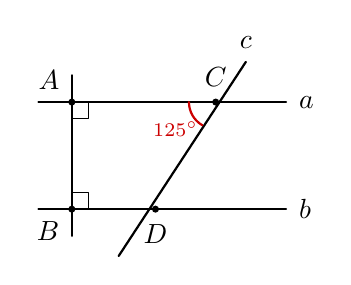
\begin{tikzpicture}[scale=0.85, >=stealth, line join=round, line cap=round]
  % Doan thang AB vuong goc
  \draw[thick] (0.8, 0.2) -- (0.8, 2.6);
  % Duong thang a qua A
  \draw[thick] (0.3, 2.2) -- (4.0, 2.2) node[right=1pt] {$a$};
  % Duong thang b qua B
  \draw[thick] (0.3, 0.6) -- (4.0, 0.6) node[right=1pt] {$b$};
  % Cat tuyen c
  \draw[thick] (3.4, 2.8) node[above=1pt] {$c$} -- (1.5, -0.1);
  
  % Giao diem A va B
  \fill (0.8, 2.2) circle (1.5pt) node[above left=1pt] {$A$};
  \fill (0.8, 0.6) circle (1.5pt) node[below left=1pt] {$B$};
  % Ky hieu vuong goc
  \draw (0.8, 1.95) -- (1.05, 1.95) -- (1.05, 2.2);
  \draw (0.8, 0.85) -- (1.05, 0.85) -- (1.05, 0.6);
  
  % Giao diem C va D
  \fill (2.95, 2.2) circle (1.5pt) node[above=2pt] {$C$};
  \fill (2.05, 0.6) circle (1.5pt) node[below=2pt] {$D$};
  
  % Goc tu ACD
  \draw[red!80!black, thick] (2.95, 2.2) ++(180:0.4) arc (180:240:0.4);
  \node[red!80!black, font=\scriptsize] at (2.35, 1.8) {$125^\circ$};
\end{tikzpicture}
\end{minipage}\par
\vspace{0.4mm}
\noindent\textit{Bài giải:}\dongkeHaiCot{10}
\\ \hline
\end{tabularx}

\vspace{1.5mm}

\noindent
\begin{tabularx}{\linewidth}{|X|}
\hline
\vspace{0.5mm}
\textbf{Câu 14 (0,5 điểm).} Cho biểu thức: $S = \dfrac{1}{2} + \dfrac{1}{2^2} + \dfrac{1}{2^3} + \dots + \dfrac{1}{2^{2026}}$. Chứng minh rằng $S < 1$.\par
\vspace{0.4mm}
\noindent\textit{Bài giải:}\dongkeHaiCot{6}
\\ \hline
\end{tabularx}

\newpage
\end{document}